\documentclass[letterpaper,12pt]{article}

\usepackage[margin=1.0in]{geometry}
\usepackage{multirow}
\usepackage{tikz}
\usepackage{amsmath}
\usepackage{hyperref}
\usepackage{pdfpages}
\usepackage{standalone}

\usetikzlibrary{shapes.geometric, arrows, fit}

\setlength\parindent{0pt}

\newcommand{\specialcell}[2][c]{\begin{tabular}[#1]{@{}c@{}}#2\end{tabular}}
\newcommand{\xxx}[1]{{\color{red}\bf #1}}
\newcommand{\AxisRotator}[1][rotate=0]{\tikz [x=0.25cm,y=0.60cm,line width=.2ex,-stealth,#1] \draw (0,0) arc (-150:150:1 and 1);}

\begin{document}

\title{\textbf{EE 4388 Senior Design II\\Semester Report}}
\author{Hazen Eckert \hspace{3mm} Omar Hasan \hspace{3mm} Ryan Marcotte \hspace{3mm} Ridhwaan Rahman}
\date{May 11, 2015}
\maketitle

\begin{center}
    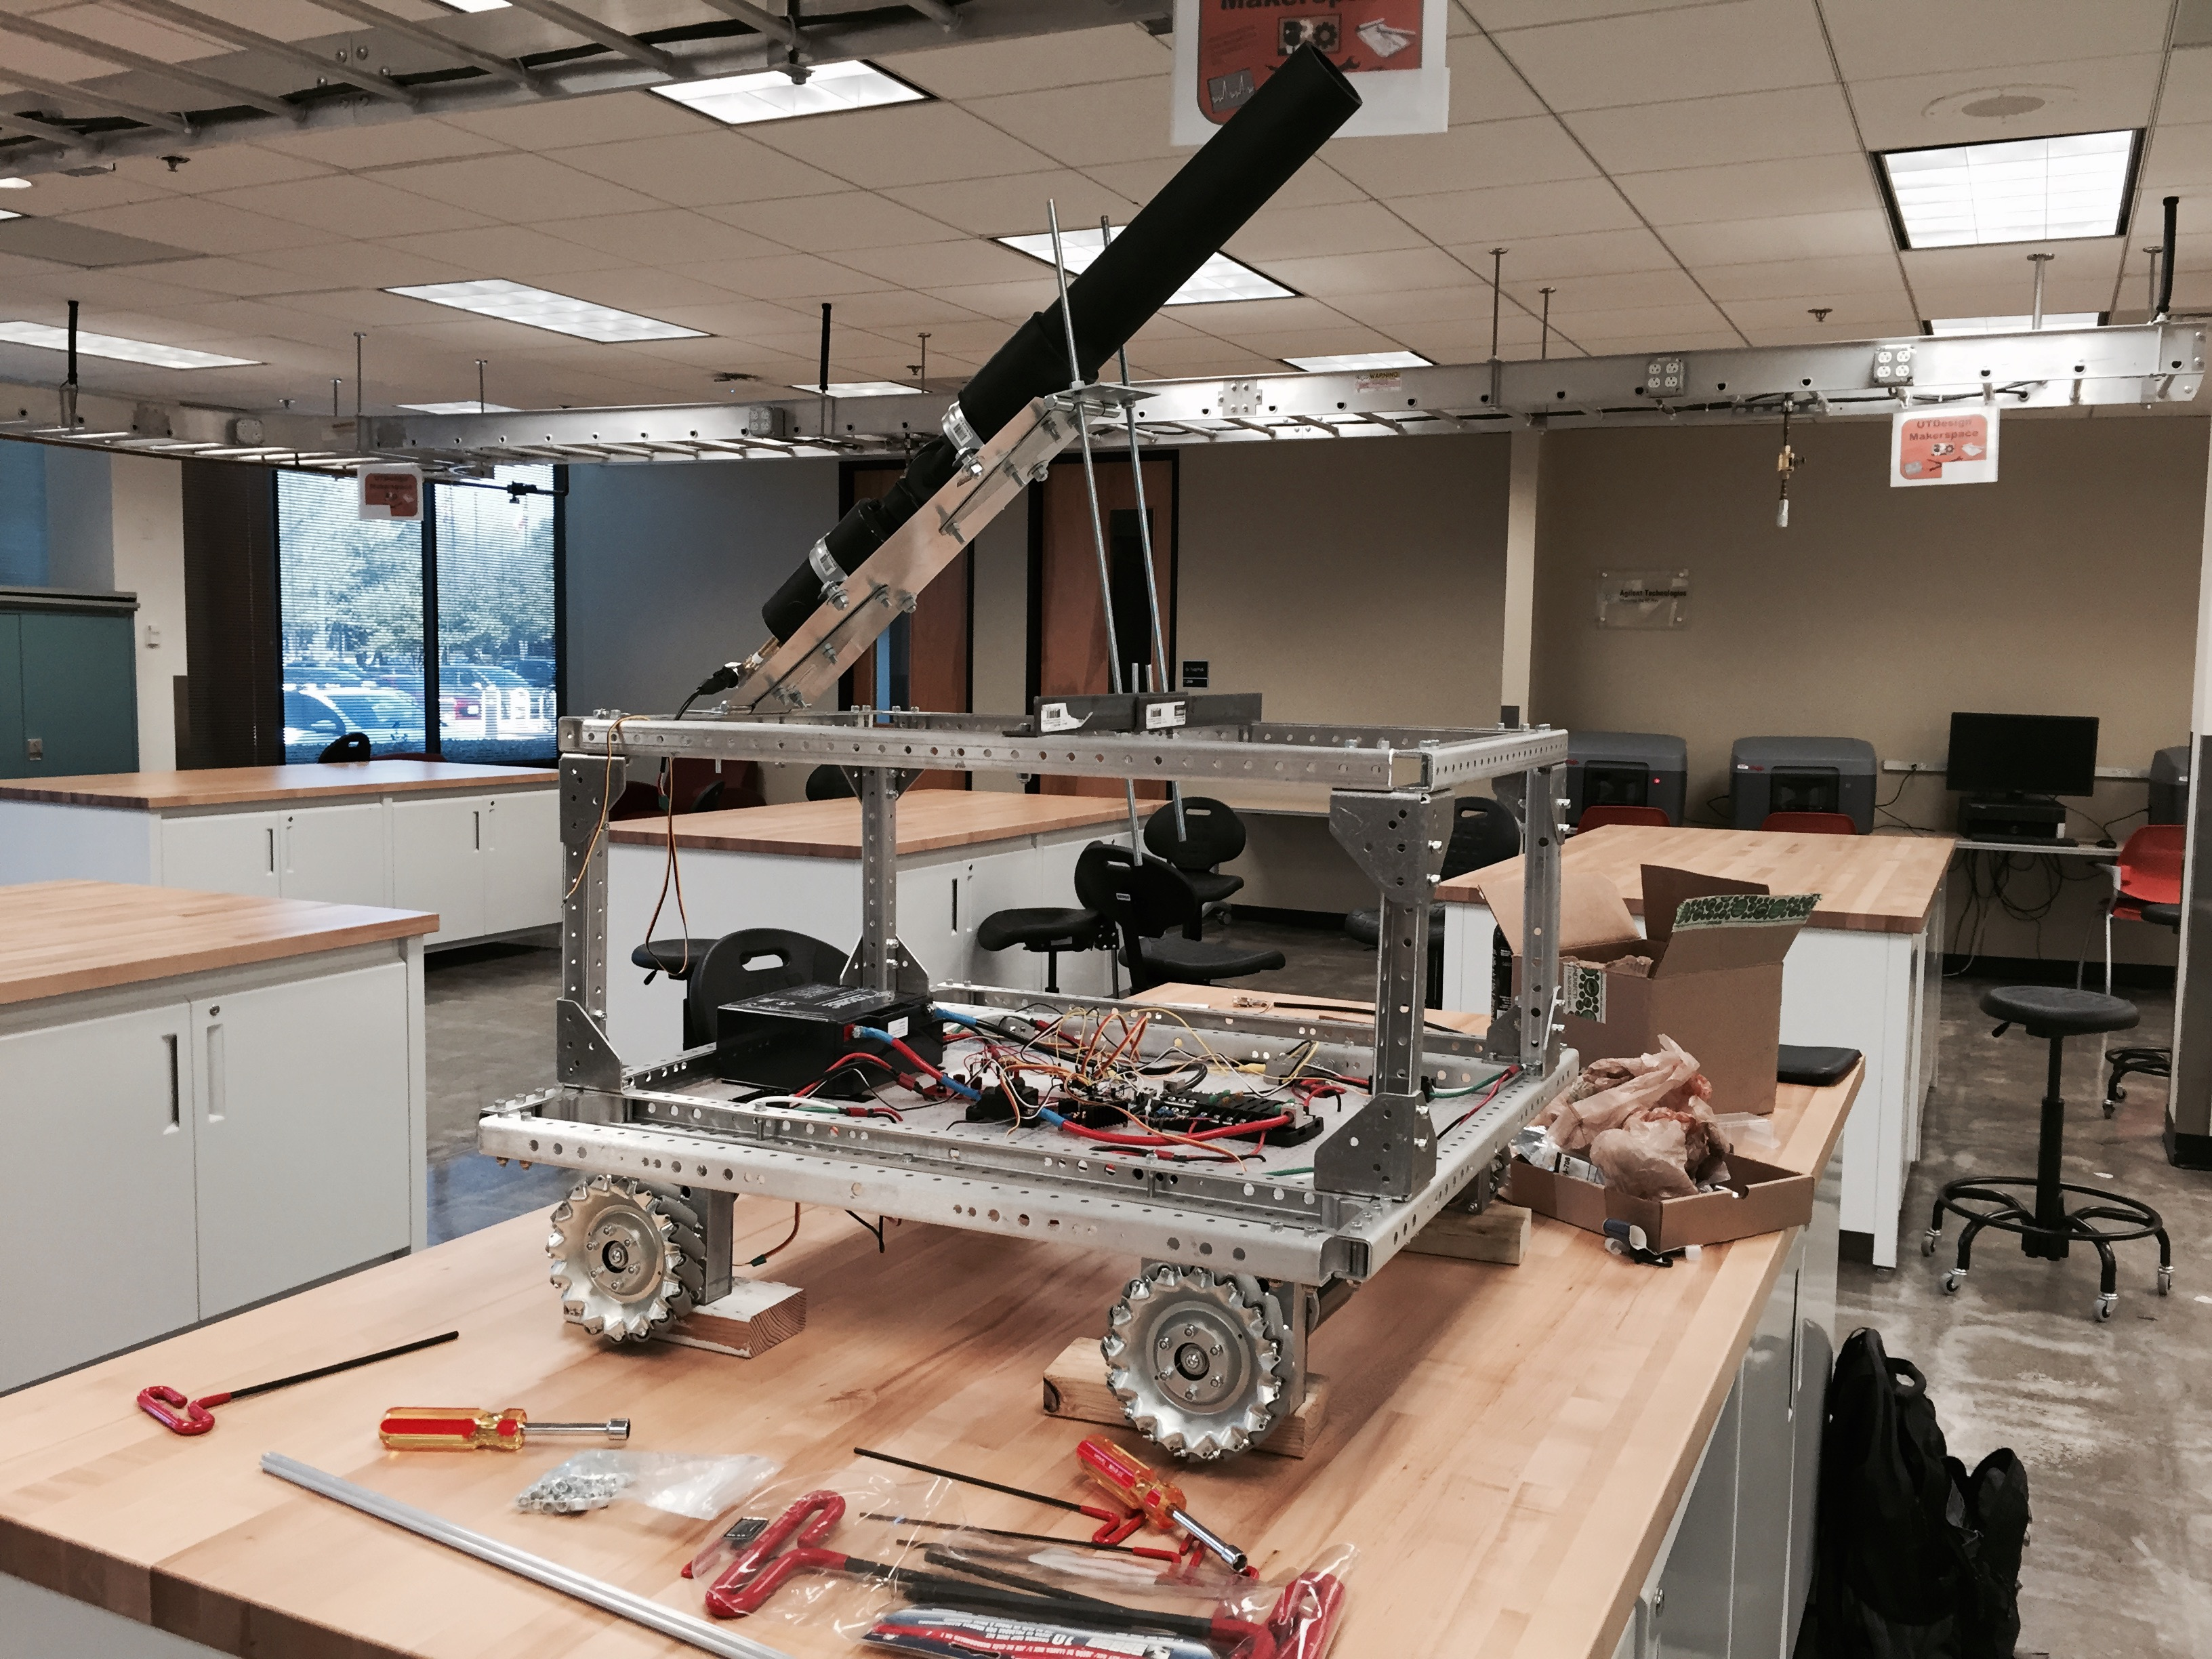
\includegraphics[width=15cm]{./pics/chassis/robot.jpg}
\end{center}

\pagebreak
\tableofcontents
\pagebreak

\section{Introduction}
\label{sec:intro}

\subsection{Purpose}
\label{sec:purpose}
Our task was to design a teleoperated, wheeled mobile robot that can launch
t-shirts safely at university events. The primary purpose of the robot will be
to promote the Erik Jonsson School of Engineering and inspire undergraduate
engineering students to gain hands-on experience with university-sponsored
engineering projects.

\subsection{Problem Statement and Design Objectives}
\label{sec:probstatement}

The design will meet the following objectives:
\begin{itemize}
    \item Operation time \textgreater 10 minutes
    \item Remote control for up to 50 feet
    \item User control of robot velocities and cannon triggering mechanism
    \item Fire t-shirts between 20 and 150 feet
    \item Send live video stream of the robot's First Person View back to the user
\end{itemize}

\subsection{Design Process Summary}
\label{sec:designprocesssummary}
We began designing our robot by determining that the drive system would be
a 4-wheel omnidirectional drive with a t-shirt launching mechanism attached
rigidly to the robot's chassis. Then, a t-shirt launching mechanism was chosen.
An electrical system for wirelessly receiving and transmitting commands and
controlling the robot's movements and t-shirt launching mechanism was designed.
Finally, a software system for handling the robot-user interface was designed.

\subsection{Final Results Summary}
\label{sec:resultssummary}
Our robot meets the specifications that were put forth in the earlier
subsections. It has been tested already on numerous occasions and has performed
the desired tasks on those occasions.

\section{Review of Conceptual and Preliminary Design}
\label{sec:conceptualpreliminarydesign}

\subsection{Problem Analysis}
\label{sec:probanalysis}
The robot must wirelessly receive and perform velocity and t-shirt launching
commands. To perform the commands, the robot must first have a mechanism by
which to control its velocity and also a triggering mechanism for the t-shirt
launcher. The robot must have a wireless receiver on-board and a camera for
first person view streaming. A central controller should coordinate all robot
tasks on-board and a power source for both the t-shirt launching mechanism as
well as the components dedicated to maneuvering the robot. The following
specifications will solve the problem as thus described:

\begin{itemize}
    \item 4-wheel omnidirectional drive
    \item Pneumatic t-shirt launcher with a shot range between 20 and 150 feet
    \item Single power source for all electrical components
    \item Single microcontroller board that includes a microcontroller and
        a microprocessor for embedded linux and wireless communication
    \item Highly reconfigurable IP camera
\end{itemize}

\subsection{Decision Analysis}
\label{sec:decisionanalysis}
We decided for the robot to have 4-wheel omnidirectional drive to allow the
user ease of control over the robot's pose. In this configuration, the user
will be able to separately control the robot's angular velocity and
translational velocity to achieve the desired pose. We chose this configuration
over others because it is simpler to implement and pre-existing solutions are
readily available at certain vendors.\\

The robot's original application is to be used during the halftime of
basketball games to entertain the crowd. Given the size of UTD's basketball
court and bleachers, a shot range between 20 and 150 feet is reasonable for
this application. For convenience, a pneumatic cannon capable of firing single
shots is a widely available commodity that can be retrofitted for our purposes.\\

A single power source would be ideal for powering the robot's 4 motors,
microcontroller, and other electronic devices. We decided to go with a single
power source and use up-conversion and down-conversion voltage regulators
rather than using multiple power sources.\\

A central microcontroller is needed to control the robot's motion and
triggering mechanism. Furthermore, since the robot will need to take wireless
commands as input, it would be ideal to wirelessly program the robot's
microcontroller as well. We chose this solution over using separate
microcontrollers for high and low level commands.\\

\section{Basic Solution Description}
\label{sec:basicsoldesc}

Our solution is most easily subdivided by the mechanical, electronic, and software solutions. The following sections will discuss each of these in turn and define their major sub components. 

\subsection{Mechanical System}
The mechanical system consists of three main components: the wheelbase, the chassis, and the cannon. The wheelbase includes the wheels, gearboxes and motors that provide movement to the chassis. The requirements that applied to the wheelbase were that it must provide holonomic movement, be safe on gym floors, and reach a maximum speed of 10 ft/s. The chassis provides the frame to which the wheelbase and cannon must mount and mounting area for all the electronics. There were only two requirement for the chassis: that it have a maximum carrying capacity of greater than 60 lbs and it would provide many mount points for future additions. Finally, the cannon is the component responsible for launching the t-shirts into the air. It was required to shoot at a select-able range from 20 to 150 feet and have a capacity of 20 shots at max range. A major requirement for our cannon was that it must be safe. To that end, we required our cannon to have an automatic pressure release system and that all pressurized components not be made with PVC because of its shattering properties. Furthermore, the cannon had to be electronically triggered and the range had to be electronically controlled. 

\begin{center}
    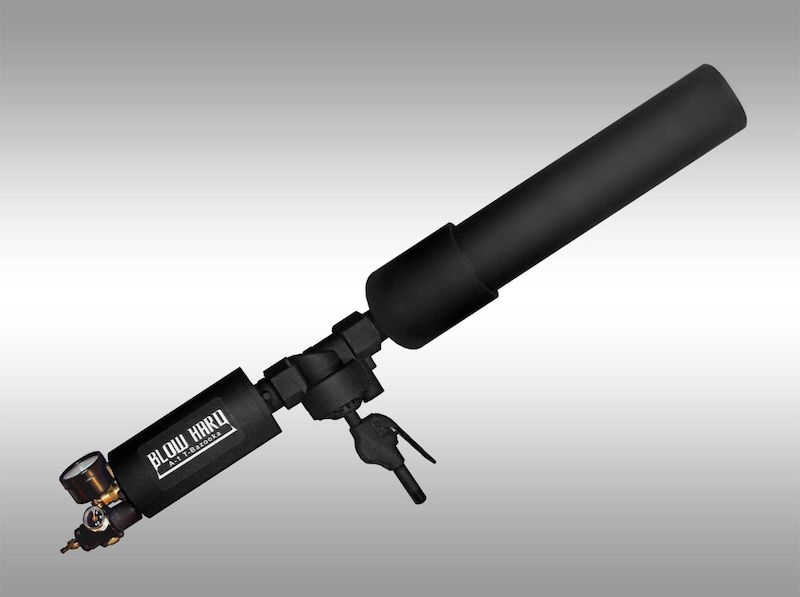
\includegraphics[width=15cm]{./pics/cannon/blowhard_cannon.jpg}\\
     Figure 1:The Blow Hard T-Shirt Cannon
\end{center}

\begin{center}
    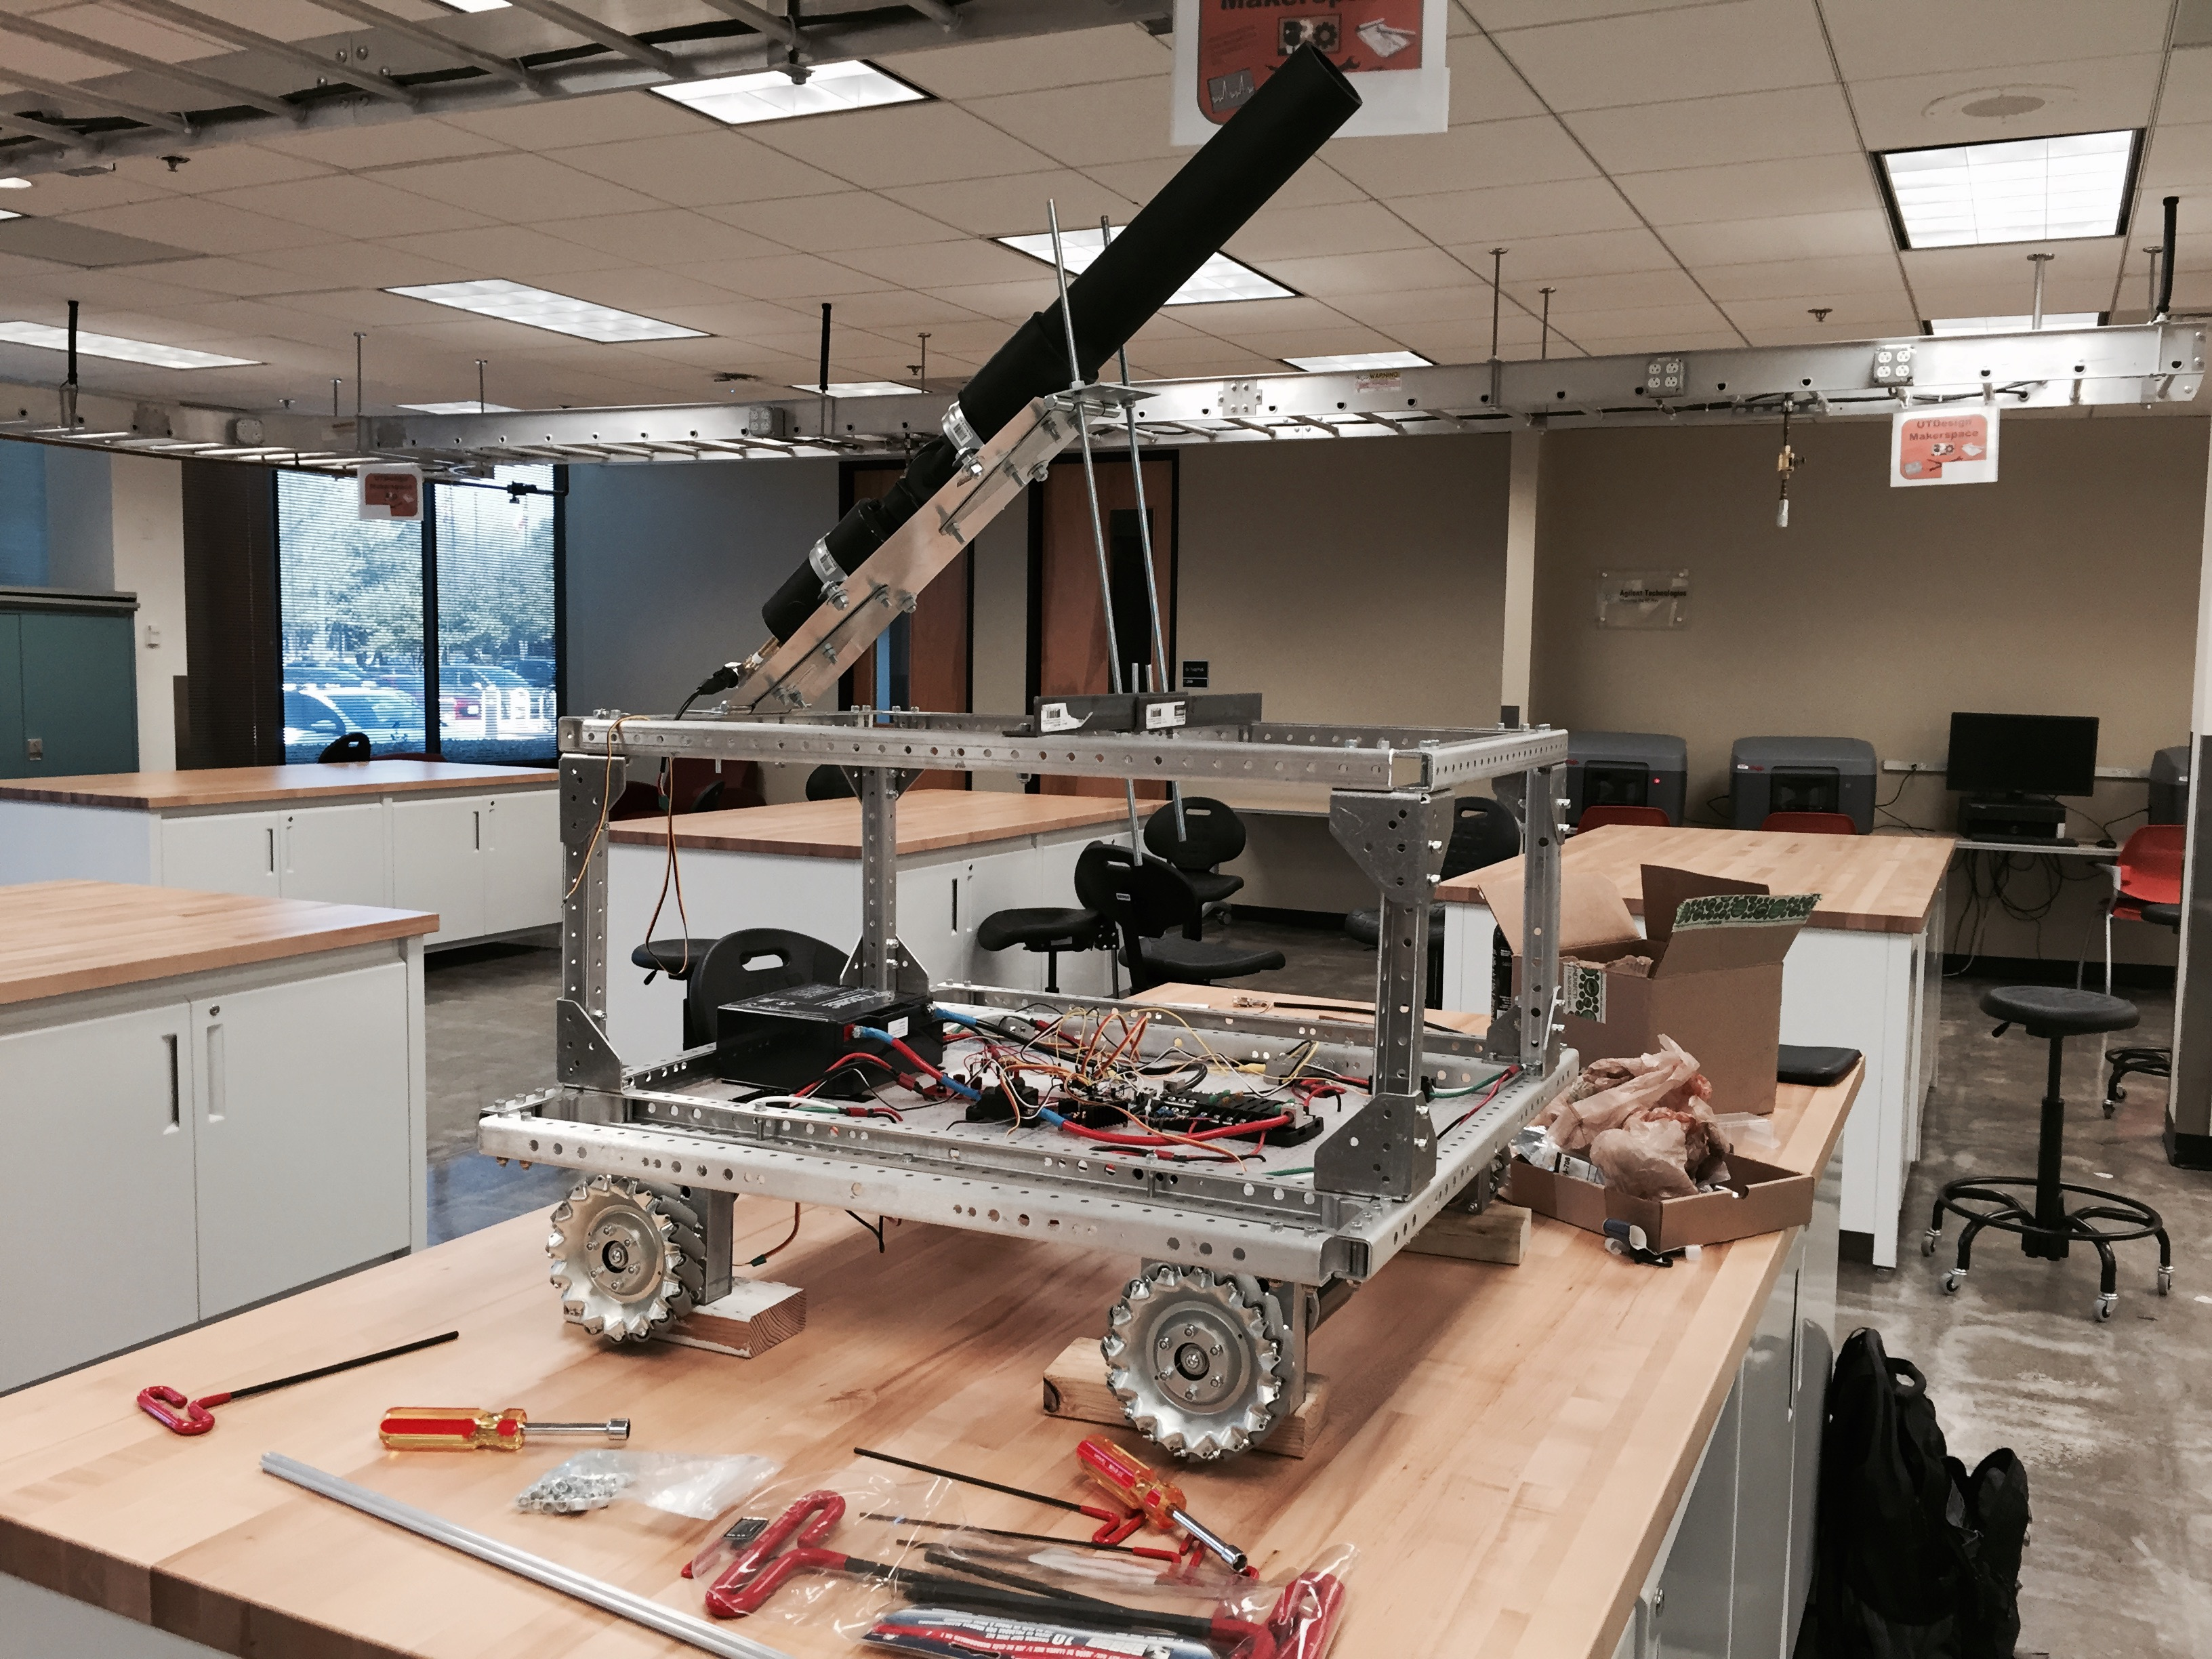
\includegraphics[width=15cm]{./pics/chassis/robot.jpg}
    Figure 2: Complete Mechanical System
\end{center}

\subsection{Electrical System}
There are many different electronic subsystems that make up the electrical system of the robot. First the power subsystem provides three different voltages (5 VDC,  12 VDC, and 24 VDC) for the other electronics. It consists of a 12 VDC battery, a boost converter to supply 24 VDC and a buck converter to supply 5 VDC. The main requirement for the power subsystem was to have enough power for at least 10 minutes of high activity usage. Beyond that requirement, our 24 VDC electronics demand at least 1.5 A and our 5VDC electronics require at least 2 A.

The control subsystem consists of the two logic boards that provide the processing power for the on board software. The Arduino Yun runs the control software and controls all the other electrical components on the robot except the camera. The Raspberry Pi controls the video stream and hosts the wireless network. These boards communicate with the user base station to receive commands and to present the user with feedback. The requirement for this subsystem was that it should be able to receive command from at least 50 ft away from the base station while streaming video and 100 ft without the video stream. 

The remaining electronics are the control circuits for the mechanical system. The electronic speed controllers (ESCs) allow the Arduino Yun to control the drive motors. The 24 VDC pneumatic solenoids provide electronic triggering and pressure regulation and their controls circuits allow the Arduino Yun to activate them. The pressure sensor provides feedback to the Arduino Yun for pressure regulation.  Encoders, which are present but not implemented for reasons explained in Section 4.2, provide wheel rotation information back to the Arduino for velocity control. Finally, a piezo buzzer acts as a horn. There were no specific requirements for these components as they were constructed as solutions to meet other requirements.

\begin{figure}[h!]
  \centering
  \includestandalone[width=0.8\textwidth]{./tikz-figures/electroncs-overview}
  \caption{Electrical System Diagram}
  \label{fig:e_system}
\end{figure}

\subsection{Software System}
The software that implement all the robots functionality can be divided up based on the physical device on which each component runs. First, the software on the ATmega that resides on the Arduino Yun is responsible for controlling the physical hardware through the on board electronics. It communicates with the Arduino Yun's Atheros chip that runs the Linux-based OpenWRT. The ATmega responds to commands from the Atheros to set the velocity of the robot, trigger and charge the cannon, and provide diagnostic information such as tank pressure. The software on the Atheros chip is mainly responsible for relaying commands from the base station to the ATmega and providing status updates to the bases station from the ATmega. 

The Raspberry Pi is configured to provide the wireless network to which the base station and Arduino Yun connect. It is additionally responsible for providing a live video stream from the robot to the base station. The base station, which consists of a Linux or Mac-based laptop and an Xbox controller, provides the user with and intuitive controller-based interface for controlling the robot and graphical user interface to provide the video stream and robot status information.

\begin{figure}[h!]
  \centering
  \includestandalone[width=0.8\textwidth]{./tikz-figures/software-overview}
  \caption{Software System Diagram}
  \label{fig:system_diagram}
\end{figure}


\section{Performance Optimization and Design of System Components}
\label{sec:optimization}

\subsection{T-Shirt Cannon}
The requirements for our cannon are that it should be electronically
trigger-able, able to shoot a t-shirt 5 to 145 feet from a 45 degree angle,
and be able to make 15 shots on a single charge. The cannon we chose is CO$_2$
based and triggers pneumatically. Other options included a mechanical throwing
mechanism or building the cannon ourselves, but those options would have taken
too much time away from designing the other components. A 20oz CO$_2$ tank
provides enough capacity for at least 15 shots at maximum range. In order to
trigger electronically, we replaced the manual pneumatic trigger with
a 2-position normally closed 1/4in solenoid valve. An electronic regulator would not fit within our budget so we
decided to use a 200 psi pressure transducer and a 2-position normally closed 1/4in solenoid valve to allow us to set
the firing pressure of the cannon, and by extension the range, electronically. As shown in the figure below, the
pressure transducer provides the current pressure in the cannon's reservoir and
the solenoid valve allows us to shut off the flow of CO$_2$ once the desired pressure
is achieved. The solenoid control circuits for both the electronic triggering and electronic pressure regulation are implemented on a prototyping board mounted on the Arduino Yun. For more information about the prototyping board see section 3.3 Control Electronics below.\\

\begin{center}
    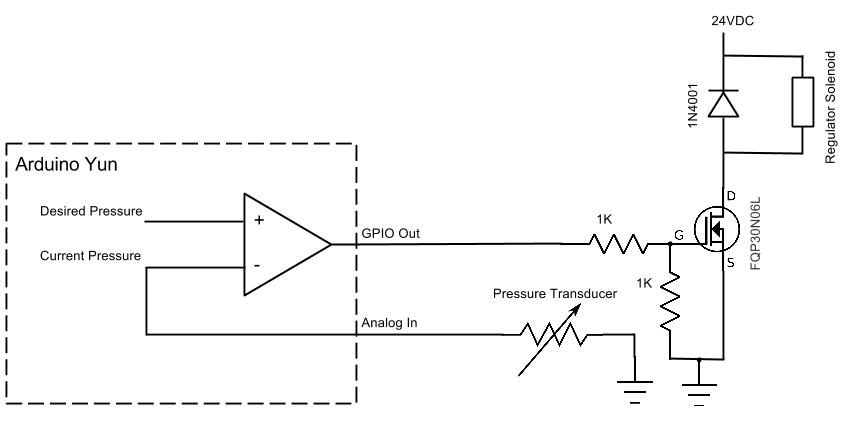
\includegraphics[width=15cm]{./pics/cannon/PressureControl.jpg}\\
     Figure 1: Electronic Pressure Control Diagram
\end{center}

\subsection{Chassis}
The original requirements for the chassis of our robot were that it had to move 
holonomically, have maximum speed of approximately 10
ft/s, be safe for gymnasium floors, and have a load capacity of approximately
60 pounds. This led us to choose a four wheeled mecanum drive
system mounted on an aluminum chassis. We chose mecanum wheels because they
have the highest load capacity and simplest control algorithm of the holonomic
drive solutions we could afford. Mecanum wheels have rollers attached at an
angle around the wheel. The wheels can operate like a screw and enable lateral
movement and rotating in place. This comes at the cost of a loss of efficiency
and each wheel requires a separate motor, gearbox, quadrature encoder, and
motor controller.\\

The motors and gearboxes that came with the chassis provide enough
torque to achieve a maximum of about 8.8 ft/s, less than the required 
10 ft/s. After testing, we determined that 6 ft/s was a safer and more 
appropriate maximum speed for our robot so we did not pursue achieving 
10 ft/s.  Originally, in order to eliminate expected drift and provide
smoother controls, we had decided to include quadrature encoders to provide
velocity feedback for a closed loop control loop. After test driving the robot and 
finding it very easy and intuitive to drive, we determined that this feature would 
not add any discernible improvement to the driver's ability 
to control the robot. Therefore, we did not add a feedback mechanism to the 
control of the robot. The motor controllers we chose can provide 40A continuous 
current to each motor, however, our power
distribution system is only capable of delivering 30A to each motor.\\

\subsection{Control Electronics}
An Arduino Yun microcontroller provides the robot with a network
connection and a low level microcontroller. Other options included Texas
Instruments based microcontrollers, but because we wanted simplicity of
programming, we went with the Arduino. The Yun has both an ATmega
microcontroller for low level control as well as an Atheros microprocessor chip
that runs OpenWrt Linux that provides networking capabilities. The Atheros runs
our application that receives velocity, triggering, and other commands over
WiFi and processes them into low level commands for the ATmega. The ATmega
handles hardware interrupt, monitors electrical components, and executes
commands given by the Atheros device. Connected to the ATmega through a prototyping board are the motor
controllers, which are controlled via PWM, the pneumatic circuits,
which provide electronic triggering and range adjustment, and a control circuit for a piezo buzzer that acts as a horn. The prototyping board is pictured below.\\

\begin{center}
    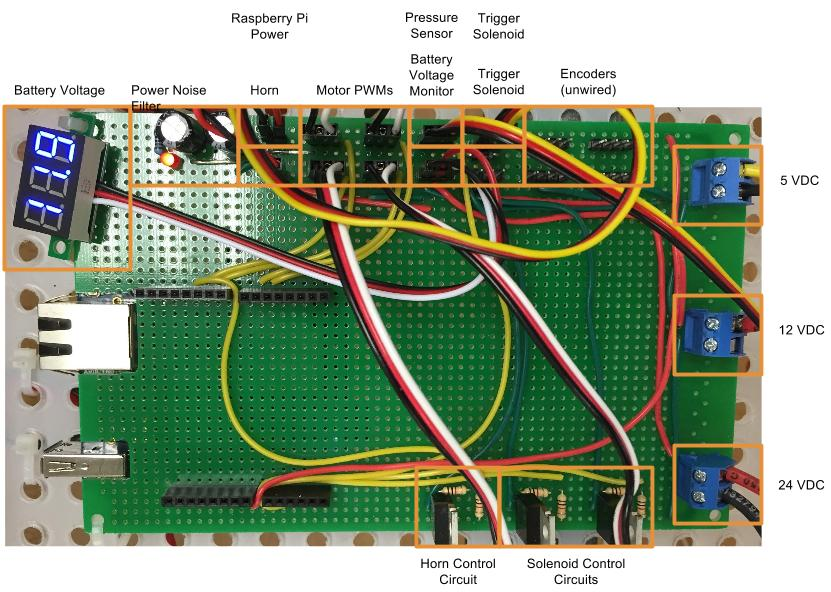
\includegraphics[width=15cm]{./pics/electronics/AnnotatedProtoboard.jpg}\\
     Image 1: Prototyping Board
\end{center}

A Raspberry Pi single board computer provides wireless networking and video 
streaming to the robot. Originally, the network was hosted by the Arduino Yun. 
However, testing revealed that the signal strength of the Yun's network did not satisfy 
our design requirements.  The network was then hosted by the Raspberry Pi using 
an USB wireless adapter with a stronger antenna. This enabled us to achieve a maximum 
range of 75ft with a video stream and 150ft without a video stream.

In the software of the control electronics are several safety power shutoffs.
If communication ceases between the Atheros and the ATmega or between the user
and the Atheros, the robot with shut off the motors. This is achieved through
a “heartbeat“ protocol, which resets a timer every time a message is received.
If no message is received before the timer expires, the connection is assumed
lost and power is shut off.\\

\subsection{User Interface}
The user interface runs on a personal computer running any operating system
with a Java Virtual Machine. An X-Box controller provides the user with
a familiar and intuitive control scheme. The graphical user interface running
on the personal computer updates the user with diagnostic information such as
current firing pressure, desired velocity, and connection strength. This
interface also presents the user with a video stream from the robot’s point of
view. The Linux-based Raspberry Pi is streaming this
video from a webcam on the robot.\\

\subsection{Power Distribution System}
The electronic devices on the robot require three different voltages: the
pneumatic components must have 24VDC, the motors need 12VDC, and the control
electronics operate at 5VDC. Since the majority of the current would be drawn
at 12V we chose a 12VDC lead acid battery and used a buck converter to obtain
5VDC and a boost converter to achieve 24VDC. A common automotive fuse box is
used to distribute the 12VDC power among up to 12 circuits at up to 30A. The
battery is able to source up to 300A at any time and can source 60A for 10
minutes straight before discharging. Since our motors will draw at least 2A at
free current, we expect that once the robot achieves a constant velocity, each
motor will draw around 10A. Thus, we expect our battery to give us enough power
to allow the robot to operate for approximately 40 minutes at a time under moderate usage.\\

A 120A breaker serves as the main power switch for the robot. The user is able to completely disconnect the robot from power by pressing the reset button on this breaker. 



\section{Performance Optimization and Design of System Components}
\label{sec:optimization}
\xxx{Description of components and their component-level specifications} \\
\xxx{Design criteria used} \\
\xxx{Discussion of the technical approach used} \\
\xxx{Discussion of design details} \\
\xxx{Presentation and discussion of engineering drawings and schematics} \\
\xxx{Fabrication, construction, or production instructions and specifications} \\
\xxx{This section should provide any and all information necessary to ``build'' the component of the design you have focused on, all the way down to the number of nuts, bolts, transistors, wiring harness pin-outs, etc.} \\
\xxx{Summary of the final design results} \\
\xxx{Performance evaluation}

In order to command a desired robot velocity,
\begin{math}
  v=
  \begin{bmatrix}
    v_x \\
    v_y \\
    \omega_z
  \end{bmatrix}
\end{math}
, we calculate the wheel velocities as shown in Equations \ref{eq:rw_to_v}-\ref{eq:v_wheel_4}, according to Figure \ref{fig:robot_top_view}.

\begin{figure}[h!]
  \centering
  \includestandalone[width=0.5\textwidth]{./tikz-figures/kinematics}
  \caption{Top View of Robot}
  \label{fig:robot_top_view}
\end{figure}

\begin{equation}
  v_{wheel}=r_{wheel}\omega_{wheel}
  \label{eq:rw_to_v}
\end{equation}
\begin{equation}
  v_{wheel\,0}=v_x-v_y-(l_1+l_2)\omega_z
  \label{eq:v_wheel_1}
\end{equation}
\begin{equation}
  v_{wheel\,1}=v_x+v_y+(l_1+l_2)\omega_z
  \label{eq:v_wheel_2}
\end{equation}
\begin{equation}
  v_{wheel\,2}=v_x-v_y+(l_1+l_2)\omega_z
  \label{eq:v_wheel_3}
\end{equation}
\begin{equation}
  v_{wheel\,3}=v_x+v_y-(l_1+l_2)\omega_z
  \label{eq:v_wheel_4}
\end{equation}

\begin{table}[h!]
  \centering
  \begin{tabular}{| c | c |}
    \hline
    \textbf{Motor} & \textbf{Position} \\
    \hline
    0 & Forward Left \\
    \hline
    1 & Forward Right \\
    \hline
    2 & Rear Right \\
    \hline
    3 & Rear Left \\
    \hline
  \end{tabular}
  \caption{Motor Numbers}
  \label{tab:motor_nums}
\end{table}

\section{Project Implementation, Operation, and Assessment}
\label{sec:implopassess}
\xxx{Details of implementation} \\
\xxx{Operational test results} \\
\xxx{Evaluation of results relative to design criteria (how well did it do?)} \\
\xxx{What changes are suggested by design results}

\section{Final Scope of Work Statement}
\label{sec:finalscope}
\xxx{Summarize what has been done} \\
\xxx{Summarize what still needs to be done} \\
\xxx{Lessons learned and suggestions for future activities} \\
\xxx{Describe any special details of the design that only you would know} \\
\xxx{Related project management issues} \\
\xxx{Address complete system life-cycle issues (marketing, sales, service, retirement)}

\subsection{T-Shirt Cannon}
The cannon we purchased has been tested manually and can achieve the desired
range of 20 to 150 feet with a capacity of at least 20 shots. The electronic
triggering and pressure regulation components have yet to be assembled and
tested. This will be a priority task for next semester. Once this is completed
we will mount the cannon onto the chassis.\\

\subsection{Chassis, Control Electronics, and Power Distribution System}
The chassis and the power distribution system have been assembled. The control
electronics have been connected to the motors and encoder. The drive system has
yet to be tested due to either defects in the motor controllers or bugs in the
micro controller code. Next semester we hope to fix this issue and test our
maximum velocity. The closed loop control, battery monitoring, and other
software will be implemented next semester.\\

\subsection{User Interface}
\xxx{The current user interface is text based, keyboard controlled, and runs
through a wireless SSH connection to the Atheros chip. We are able to establish
communication between the Atheros and the ATmega and send commands to change
desired motor velocities. Video streaming has been achieved and can be viewed
through the browser on a computer connected to the same network as the
Raspberry Pi. Next semester we will create the user application on a personal
computer and display the video stream through that application’s graphical user
interface. We will write the server application on the Atheros that receives
messages from the user application and implement a full message protocol for
the communication between the Atheros and the ATmega and the user application
and the Atheros.}\\

\section{Cost Estimation}

\label{sec:cost}
1x Arduino Yun MCU: \$65.75 \\
1x Mecanum chassis: \$1012 \\
1x T-shirt cannon: \$365 \\
2x Lead Acid Battery: \$84 \\
1x Electronic Speed Controller: \$45 \\
1x Battery Fuse: \$50 \\
1x Power Converter: \$15 \\
1x Assorted 30A Fuses: \$5.99 \\
1x Power Distribution Board: \$38.69 \\
1x Pi Camera Module: \$26.72 \\
4x Churro Tubes: \$20 \\
4x L Brackets: \$24 \\
1x Raspberry Pi Clear Camera Case: \$8.99 \\
2x CO2 Tank: \$41.98 \\
1x 2-Way 2-pos 1/4in solenoid valve: \$56 \\
1x 150W Boost Converter: \$6.10 \\
1x 200psi Pressure Transducer: \$26 \\
25x 1n4001 diode: \$3.70 \\
10x MOSFET: \$9.14 \\

4x Victor SP Speed Controller: \$240 \\
1x AQUATEK CO2 Paintball Tank CGA 320 Adapter: \$16.99 \\
1x 1/4-20 Nylock Nut, 100 (am-1160): \$4 \\
1x 1/4-20 x 1-3/4" SHCS, 50 (am-1206): \$14 \\
2x 72" C-Channel (am-3052): \$56 \\
1x 30" C-Channel (am-2222): \$18 \\
8x Vertical Corner Link for C-Channel (am-0935): \$88 \\
1x Hitec 59411 Servo Wire 50' 3 Color \$13.41 \\
1x Easy More 15Pcs 40 Pin 2.54 mm Single Row(L 11MM) Male Header \$8.60 \\
1x Sparkfun Ribbon Cable - 10 wire (15ft) \$9.95 \\
1x Goodyear EP 46508 3/8-Inch by 3-Feet 250 PSI Lead-In Rubber Air Hose with 1/4-Inch MNPT Ends \$9.06 \\
1x Raspberry Pi 2 Model B Project Board	\$44.79 \\
1x Premium Clear Case for Raspberry Pi 2 Model B Quad Core and Raspberry Pi Model B+ \$9.49 \\
1x 8GB Sandisk MicroSDHC Memory Card with SD Adapter	\$6.49 \\
1x Wireless Xbox 360 Gaming Controller \$33.49 \\
1x Charge kit \$13.99 \\
1x TP-Link TL-WN722N Wireless Adapter \$14.99 \\

Miscellaneous (Wire, nuts, bolts, etc): \$95.37 \\

Total Cost: \$2600.68

\pagebreak

\section{Project Management Summary}
\label{sec:projman}

\subsection{Gantt Chart}
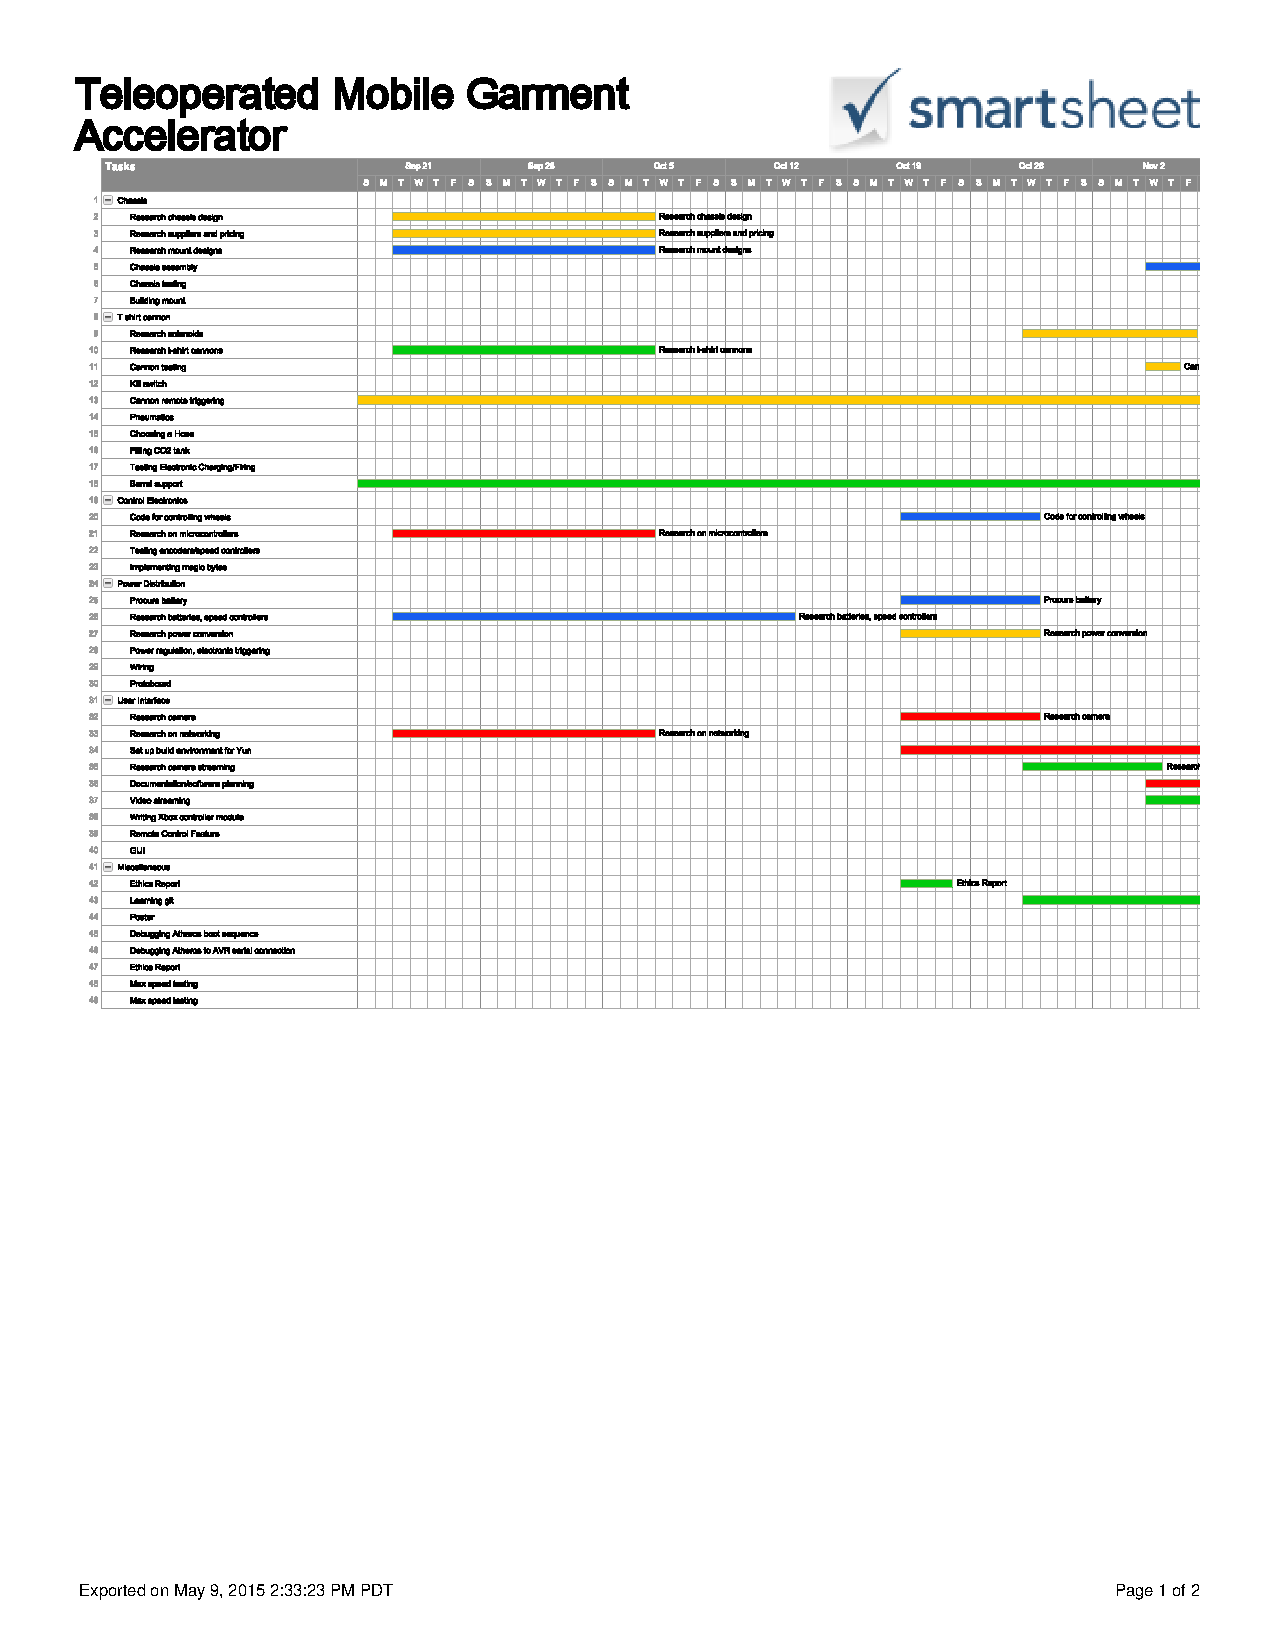
\includepdf[pages={-}]{./pics/s1.pdf}
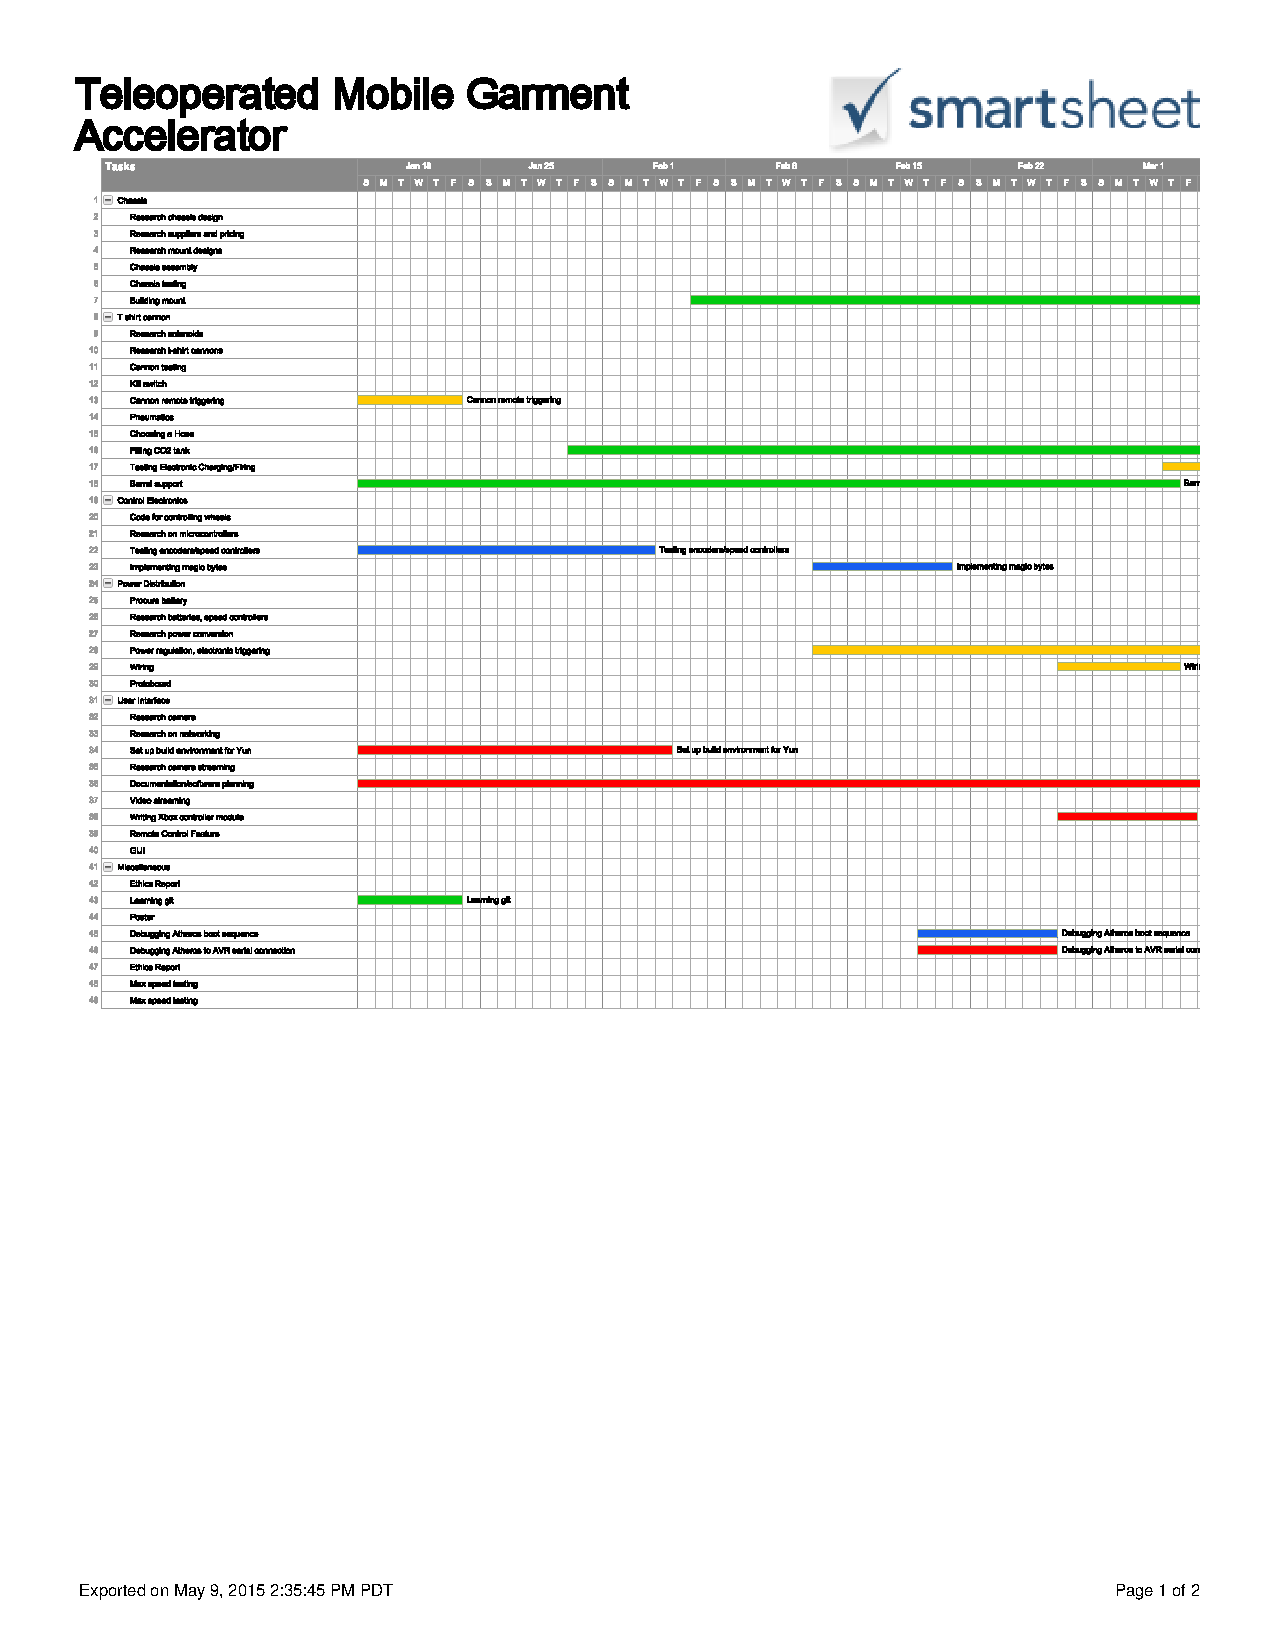
\includepdf[pages={-}]{./pics/s2.pdf}

\subsection{Work Breakdown Structure}
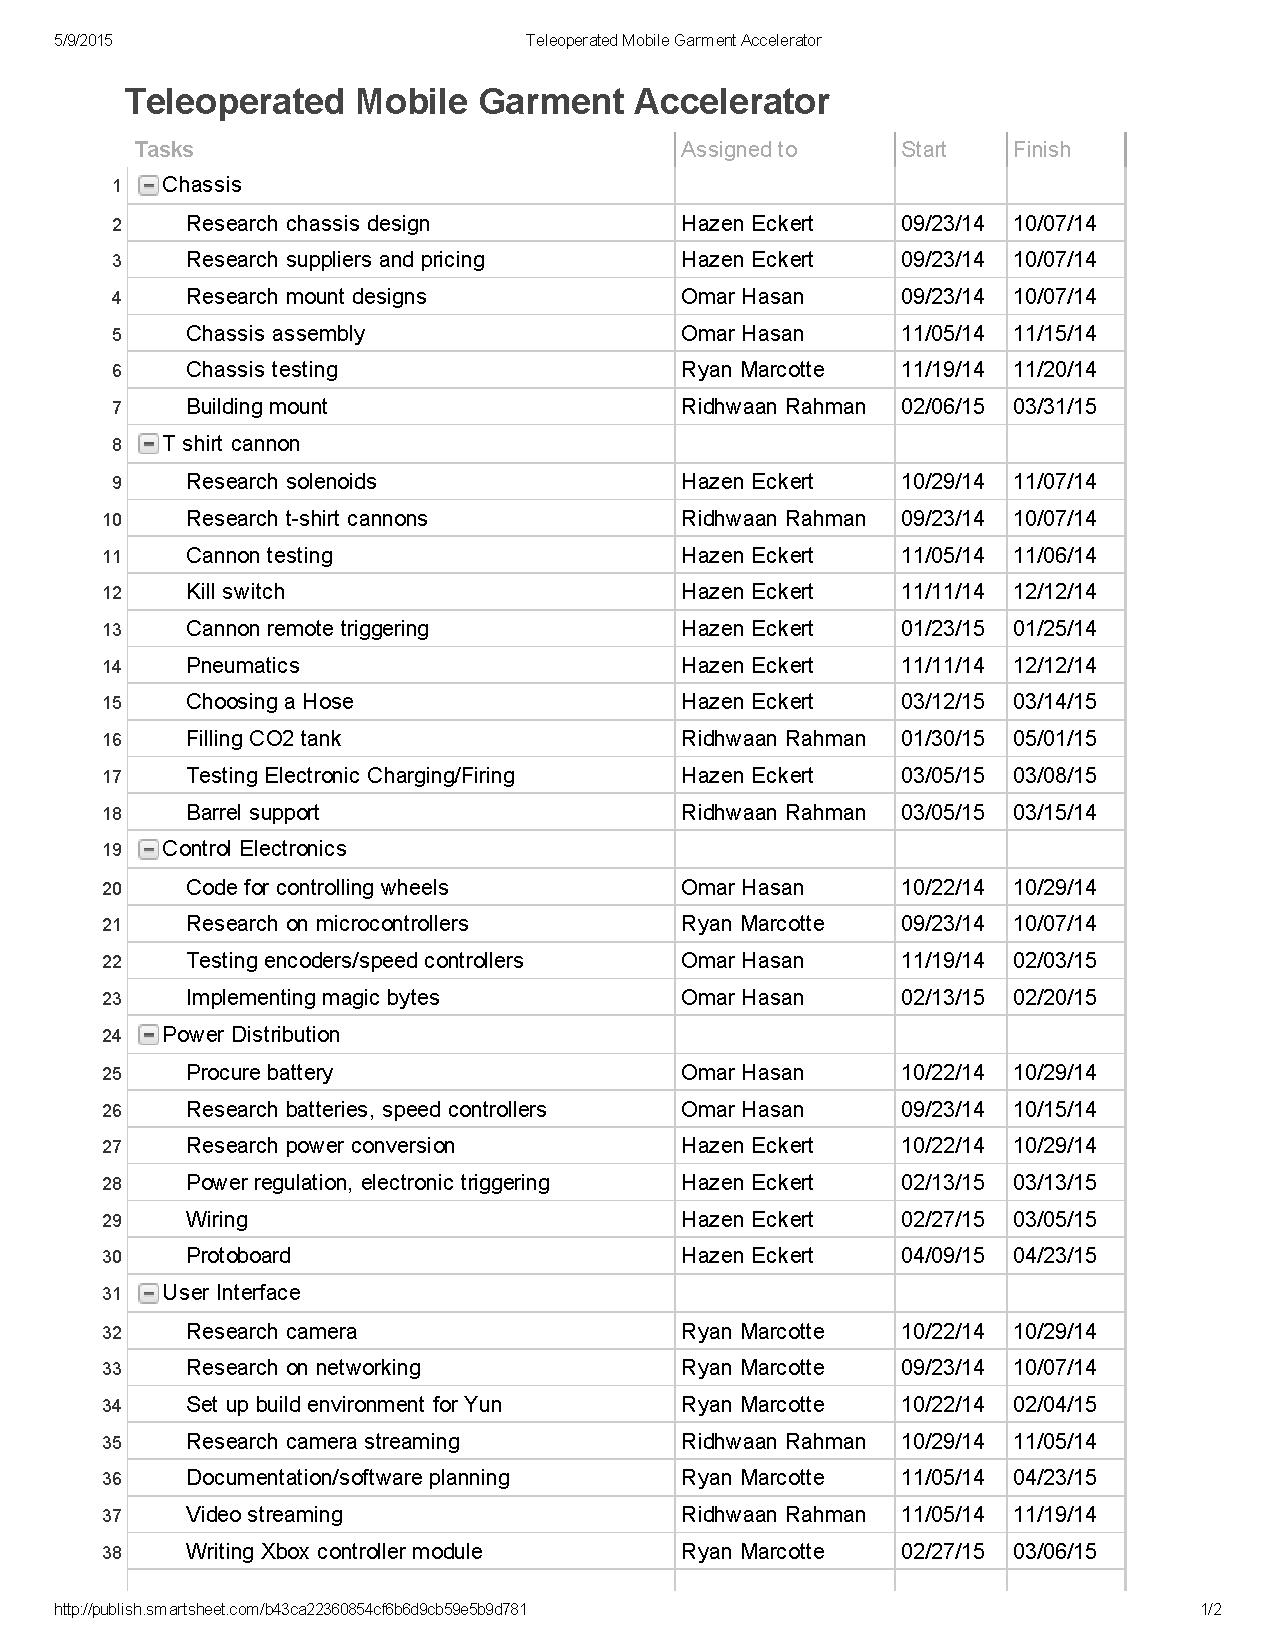
\includepdf[pages={-}]{./pics/wbs.pdf}

\subsection{Tasks}
Completed:
\begin{itemize}
    \item Pressure sensing and control of the cannon's air tank
    \item Software development on the Arduino Yun
    \item Chassis Assembly
    \item Video streaming
    \item Solenoid as triggering mechanism
\end{itemize}

Future Work:
\begin{itemize}
    \item Add reloading capabilities. Currently the cannon has to be reloaded
        manually after every shot.
    \item Modulate angle of elevation. This can be solved by implementing
        a linear actuator.
    \item Decorate the exterior. Aesthetics of the robot are being designed by
        students in ATEC.
\end{itemize}

\subsection{Time}
Two Semesters:
\begin{itemize}
    \item Weekly meetings with Dr. Gans
    \item Weekly meetings among group to organize and assign tasks
\end{itemize}

\subsection{Budget}

Our total available budget is \$3,000. Thus far we have spent \$2600.44 on
a microcontrollers, chassis, t-shirt cannon, power distribution essentials, and
pneumatics.

\subsection{Facilities}
We conducted our work in the UTDesign Lab in SPN.

\section{Conclusion}
\label{sec:conclusion}

Our sponsor and customer, the UTDesign Program, tasked us with developing
a mobile robot capable of firing soft projectiles - such as t-shirts or
confetti. This robot is to be used at sporting events, recruitment visits, and
perhaps even graduation as a way of promoting UT Dallas, the Erik Jonsson
School, and the engineering discipline in general.\\

The robot's mecanum wheels allow it to move in any direction instantaneously.
The cannon is powered by compressed CO2. We are able to remotely control the
tank's pressure and fire the cannon through the use of solenoids. The robot has
two microcontrollers on board that are networked together. An Arduino Yun
accepts and carries out commands from the user while sending a continuous
stream of diagnostic information back to the user. A Raspberry Pi and camera
module are tasked with capturing and transmitting a live video stream that can
be used for a variety of purposes, including safety mechanisms, visual
servoing, or simply entertainment. We have designed a custom protoboard to
house our electronic components. We have a variety of circuits on this board,
including power distribution, battery voltage monitoring, and control circuits
for the cannon solenoids and even a buzzer that acts as a horn.\\

The robot performs very well for its target application. The cannon has an
excellent range. We can launch t-shirts all the way across UTD's gym or we
scale back the range by decreasing the pressure in the tank. Our communication
range with the robot is limited by the mobile ad-hoc network we utilize. This
range could conceivably be increased by using existing network infrastructure,
such as the school's wireless network. However, the current network performance
is sufficient for our intended application. The robot is capable of moving
quite rapidly, so we actually have put mechanisms in place to limit its speed
due to safety and usability concerns.

\end{document}
